%
%   This file is derived from the APS files in the REVTeX 4 distribution.
%   Version 4.0 of REVTeX, August 2001
%
%   It has been simplified for use in Physics 3730/6720 by C. DeTar
%
%   Copyright (c) 2001 The American Physical Society.
%
%   See the REVTeX 4 README file for restrictions and more information.
%
% See the REVTeX 4 README file
%
\documentclass[aps,12pt]{revtex4}

\usepackage{graphicx}% Include figure files
\usepackage{bm}% bold math

\begin{document}

\title{Homework 5: LaTeX}

\author{Samir Suthar}

\affiliation{University of Utah, \linebreak Physics \& Astronomy Dept.}

\date{\today}

\maketitle

\section{Abstract}

Is it not strange that we cook bacon and bake cookies? What happens when we bake bacon and cook cookies? Results are unusual for food items.

\section{Introduction}

We tried baking bacon and cooking cookies. Our results were.....complicated. By switching how each food was cooked and creating a sort of repetition with its words, we found that the food items followed Heisenberg's Uncertainty Principle.

\section{Equations}
\begin{eqnarray}
\Delta x\Delta p \sim \hbar
\end{eqnarray}

\begin{figure}[h]
\centerline{
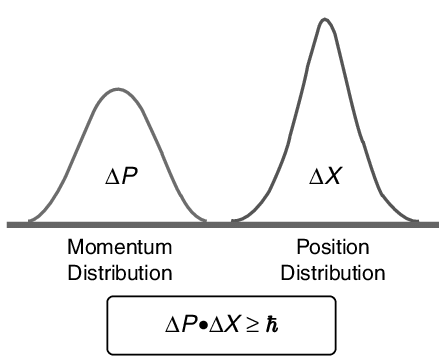
\includegraphics[width=4.5in]{Heisenberg-Uncertainty-Principle.png}
}
\caption{Heisenberg Uncertainty Principle}\label{fig:arb}
\end{figure}

\begin{thebibliography}{9}
\bibitem{knuthwebsite}
Research Gate, Keivan Esfarjani
\\\texttt{https://www.researchgate.net/figure/Heisenberg-Uncertainty-Principle\_fig4\_237677715}
\end{thebibliography}
\end{document}
